\chapter{(In)sanity check: HeartPole}
\label{ch:heartpole}

\begin{remark}
    An earlier revision \cite{heartpole} of this chapter was presented at HEALTHINF 2021. An implementation of HeartPole is available at \cite{liventsevVadim0x60Heartpole2024} 
\end{remark}

\todo{Make sure a research question is explicitly mentioned}

\section{Introduction}
\label{sec:heartpole-introduction}

Reinforcement learning in Healthcare is an emergent field that has created a demand for patient simulators like GYMIC \cite{gym-sepsis} - a black box neural model trained on MIMIC III dataset \cite{johnsonMIMICIIIFreelyAccessible2016} that predicts health outcomes of clinical decisions and can be used for training clinical decision-making models. We introduce a patient simulator inspired by \emph{CartPole} \cite{cartpole} that trades clinical accuracy off for \emph{simplicity} and \emph{transparency}, while still being \emph{non-trivial} to solve.

\section{HeartPole environment}
\label{sec:heartpole-methodology}

\begin{figure}
    \centering
    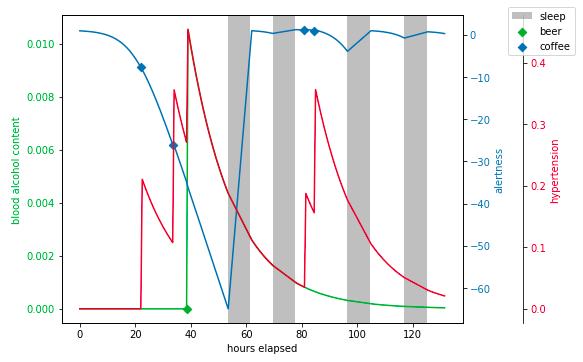
\includegraphics[width=\linewidth]{heartpole_example.png}
    \caption{Random agent's health indicators}
    \label{fig:random}
\end{figure}

\emph{HeartPole} simulates a creative professional trying to become more productive.
However, many decisions that would help in the short term (not sleeping, consuming coffee and alcohol) can create long-term health issues that negate all short term gains.

\emph{HeartPole} is a fully observable Markov Decision Process \cite{mdp} where state $\state_\step$ consists of alertness $\state^\text{alert}_\step$, hypertension $\state^\text{hypert}_\step$, intoxication $\state^\text{tox}_\step$ time since slept $\state^\text{tawake}_\step$, \emph{total time elapsed} $\state^\text{ttotal}_\step$ and \emph{total work done} $\state^\text{done}_\step$.

\begin{figure}
    \centering
    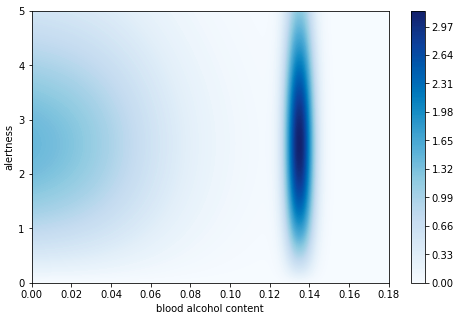
\includegraphics[width=\linewidth]{productivity.png}
    \caption{Productivity function}
    \label{fig:productivity}
\end{figure}

Over these parameters, we define \emph{productivity} function $\eta(\state^\text{alert}_\step, \state^\text{tox}_\step)$ presented graphically on figure \ref{fig:productivity} and \emph{heart attack probability} $r(\state^\text{hypert}_\step)=\frac{\text{sigmoid}(\state^\text{hypert}_\step)}{2}$.
The agent receives small positive rewards for productivity and a very large negative reward if a heart attack occurs.

Every half an hour awake, the agent observes $\state_\step$ and picks an action $\action_\step$ from discrete action space of \emph{just work}, \emph{drink coffee} (increases $\state^\text{alert}$ and $\state^\text{hypert}$), \emph{drink beer} (decreases $\state^\text{alert}$, increases $\state^\text{hypert}$ and $\state^\text{tox}_\step$) and \emph{go to bed} (sleep takes a lot of time, but reduces $\state^\text{hypert}$ and $\state^\text{tox}_\step$ and without it alertness starts to fall very fast)

\section{Reinforcement Learning}
\label{sec:heartpole-experiments}

\todo{cite deceptive diversity}

We train 2 models (a neural network with 0 hidden layers against one with 3 hidden layers of size 16) with 3 industry-standard algorithms: CEM \cite{cem}, SARSA \cite[Chapter 6]{suttonReinforcementLearningSecond2018} and DQN \cite{dqn1,dqn2} and compare the resulting agents with a reference strategy of sleep every night followed by a cup of coffee.

We train all models with \texttt{keras-rl} \cite{kerasrl}, limiting all episodes to 1000 steps, and test 20 times.
Scores in table \ref{tab:heartpole-results} are obtained by averaging over total rewards for the 20 test episodes.

\begin{table}[]
    \centering
    \begin{tabular}{c|c|c|c|c}
         Algorithm & Model & Score & Sleep & Drinks \\
         CEM & 0 & -524.12 &  &   \\
         CEM & 3x16 & -523.88 & & \\
         SARSA & 0 & -130.9 & Yes & \\
         SARSA & 3x16 & -134.95 & Yes & \\
         DQN & 0 & -119.95 & Yes &  \\
         DQN & 3x16 & \textbf{-84.96} & Yes &  \\
         Reference & - & -119.76 & Yes & Yes 
    \end{tabular}
    \caption{Reinforcement learning compared to reference strategy. All models trained to avoid caffeine and alcohol}
    \label{tab:heartpole-results}
\end{table}

We have observed that during first epochs of training the models invariably tend towards high coffee and alcohol consumption (behavior with immediate positive reinforcement but long-term negative side effects), but then converge to more conservative strategies focused on timing sleep correctly and avoiding drinks. 
This, together with the fact that only one of RL algorithms has outperformed the reference strategy supports our claim that HeartPole is \emph{non-trivial}.
At the same time it provides a high level of \emph{transparency}, making it easy to develop and analyze algorithms for reinforcement learning in Healthcare.

\newpage
\section{Program Synthesis}
\todo{Turn this into actual text}

\paragraph{Prompts}

\paragraph{Generated program}

With a Deepseek model:

\lstinputlisting{listings/metanurse-deepseek.py}

With GPT:

\lstinputlisting{listings/metanurse-gpt.py}

for 2868 iterations

\paragraph{Evaluation}

\begin{tabular}{lrr}
\toprule
model & avg score & best avg score \\
\midrule
deepseek-coder & -149.952560 & 0.400517 \\
gpt-4o & -99.885775 & 0.348758 \\
\bottomrule
\end{tabular}